\section{Wyniki}
    Ze względu na losowość początkowych wag, sieć może zwracać inne wyniki pomimo
    tych samych danych treningowych. Znacząco może różnić się także błąd. Należy
    zaznaczyć, że błąd nie ma dużego związku z wynikami które otrzymuje użytkownik
    tzn. błąd może być bardzo podobny dla dwóch przypadków ale ich wyniki będą różne.

    \subsection{Przypadek 1}
        Najczęściej występujący przypadek, przypisuje wszystkie książki danego autora
        pod warunkiem, że użytkownik polubił przynajmniej jedną:

            \begin{figure}[H]
                \centering

                Średni błąd wyniósł: $2.7799$. Wykres błędu wygląda następująco:
                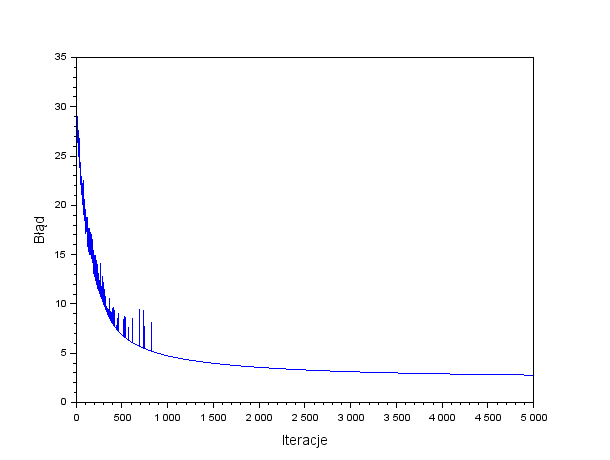
\includegraphics[width=\textwidth]{img/wykres_1.png}

                \caption{Wykres błędu w 1 przypadku}

                \label{rys:1}
                \addcontentsline{toc}{subsubsection}{Wykres \ref{rys:1}}
            \end{figure}

            Widzimy, że błąd w pewnym momencie się ustabilizował i powoli malał.

        \paragraph{}
            Po przeprowadzonym treningu podaliśmy dane wejściowe i przeprowadziliśmy test.
            W danych wejściowych użytkownik podał, że lubi:

            \textit{
                Hobbit, Krew elfów, HP: Kamień filozoficzny.
            }
        \paragraph{}
            Algorytm określił że mogą spodobać mu się:

            \textit{
                Hobbit, Władca Pierścieni, Silmarillion, Historia Śródziemia,
                Krew elfów, Czas pogardy, Chrzest ognia, Wieża Jaskółki, HP: Kamień filozoficzny,
                HP: Komnata tajemnic, HP: Więzień azkabanu, HP: Czara ognia, HP: Książę półkrwi,
                HP: Insygnia śmierci.
            }

        \paragraph{}
            Te wyniki odpowiadają temu czego się spodziewaliśmy, mamy 4 autorów oraz
            4 węzły ukryte, zakładaliśmy że sieć nauczy się rozpoznawać książkę po autorze i
            tak właśnie jest.

    \subsection{Przypadek 2}
        Czasami algorytm nie działa tak jak byśmy się tego spodziewali, w tym przypadku
        widzimy że sieć nie powiązała do końca książek z autorami, jeden węzeł ma pewną
        nieznaną dla nas zależność która zmienia znacząco wynik.

            \begin{figure}[H]
                \centering

                Średni błąd wyniósł: $3.0233$. Wykres błędu wygląda następująco:
                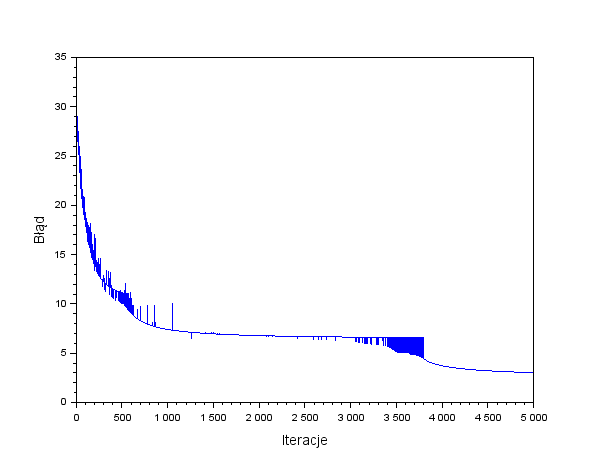
\includegraphics[width=\textwidth]{img/wykres_2.png}

                \caption{Wykres błędu w 2 przypadku}

                \label{rys:2}
                \addcontentsline{toc}{subsubsection}{Wykres \ref{rys:2}}
            \end{figure}

            W tym przypadku błąd się na krótko ustabilizował następnie znowu mocno zmieniał.


        \paragraph{}
            Po przeprowadzonym treningu (na tych samych danych) podaliśmy te same dane wejściowe
            i przeprowadziliśmy test. W danych wejściowych użytkownik podał, że lubi:

            \textit{
                Hobbit, Krew elfów, HP: Kamień filozoficzny.
            }
        \paragraph{}
            Algorytm określił że mogą spodobać mu się:

            \textit{
                Hobbit,  Władca Pierścieni, Silmarillion,  Historia Śródziemia, Przygody Toma Bombadila,
                Uczta dla wron,  Krew elfów,  Czas pogardy,  Chrzest ognia,  Wieża Jaskółki.
            }

        \paragraph{}
            Pomimo tego że użytkownik lubi książkę o \textit{Harrym Potterze} algorytm poleca \textit{Ucztę Wron}.
            W zależności od tego co chcemy osiągnąć jest to działanie niepożądane lub wręcz przeciwnie.
            Ten niespodziewany wynik pokazuje że zawsze trzeba testować swój algorytm przynajmniej kilka
            razy aby móc zaobserwować efekty których nie można przewidzieć.
